\section{DPDK(Data Plane Development Kit)}
\label{sec:DPDK}
本章では,DPDKによるパケットI/O処理とその実行モデルについて述べる.また,カーネルによるパケットI/O処理とDPDKによるパケットI/O処理の比較やDPDKによるパケットI/O処理の問題点についても述べる.

\subsection{DPDKによるパケットI/O処理}
DPDK \cite{DPDK} とは2010年にIntelによって作られたパケット処理を高速化するためのライブラリである.

DPDKは特定のCPUコアを専有することによって,NICを常時ポーリングで監視する.そのため,DPDKによるパケットI/O処理(図\ref{fig:DPDKPacketIO})では,一定時間に受信するパケットの量が増えても,コンテキストスイッチが増加することはない.

また,DPDKによるパケットI/O処理では,NICは受信したパケットをユーザ空間からアクセス可能な主記憶領域に書き込む.そのため,受信したパケットをカーネル空間からユーザ空間にコピーしなくても,ユーザ空間のアプリケーションがパケットにアクセスすることができる.

\begin{figure}[htb]
  \centering
  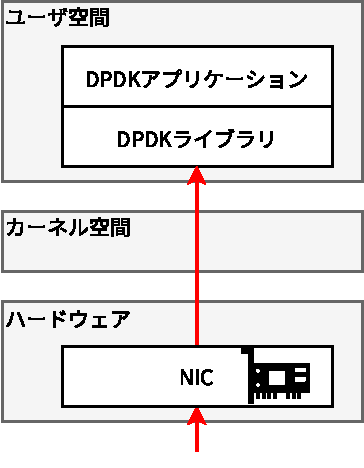
\includegraphics[width=0.5\columnwidth]{pictures/DPDKPacketIO.pdf}
  \caption{DPDKによるパケットI/O処理}
  \label{fig:DPDKPacketIO}
\end{figure}

\subsection{DPDKの実行モデル}
DPDKの実行モデルにはRun-to-CompletionモデルとPipelineモデルの二つがある.Run-to-Completionモデルは受信処理,パケット処理,送信処理を一つの論理コアで行うモデルである(図\ref{fig:RunToCompletion}).パケット処理が重い場合は受信処理にCPUリソースが割り当たらず,パケットロスが生じるため,パケット処理ではパケットヘッダの書き換えといった軽い処理が一般的には行われる.Pipelineモデルは受信処理,パケット処理,送信処理をそれぞれ別の論理コアで行うモデルである(図\ref{fig:Pipeline}).受信処理を行う論理コアとパケット処理を行う論理コアが別であるため,パケット処理が重い場合でもパケットロスが生じることはない.しかし,それぞれの処理が論理コアを専有するため,CPUリソースやパケット処理時に必要なデータの大部分がL1キャッシュに存在し,結果として処理速度が向上するという効果を有効活用できない.

\begin{figure}[htb]
  \centering
  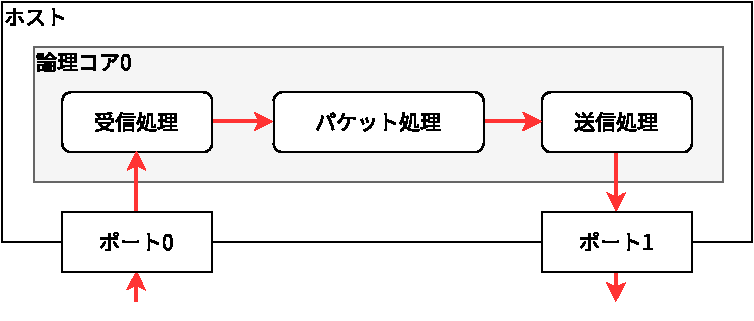
\includegraphics[width=\columnwidth]{pictures/RunToCompletion.pdf}
  \caption{Run-to-Completionモデル}
  \label{fig:RunToCompletion}
\end{figure}

\begin{figure}[htb]
  \centering
  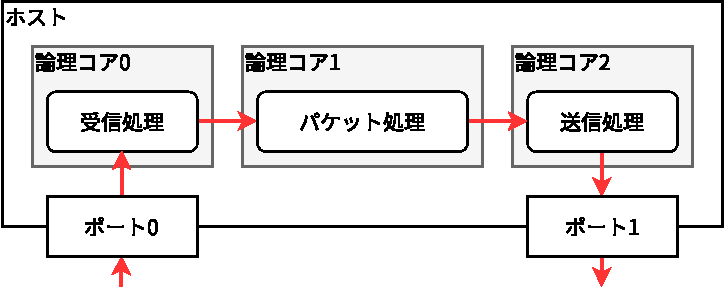
\includegraphics[width=\columnwidth]{pictures/Pipeline.pdf}
  \caption{Pipelineモデル}
  \label{fig:Pipeline}
\end{figure}

\subsection{パケットI/O処理の比較}
文献 \cite{XDP} で調査された,Linux4.18のカーネルによるパケットI/O処理とDPDKによるパケットI/O処理の通信スループットを図\ref{fig:PacketIOComparison}に示す.このグラフの横軸は使用したCPUコアの数,縦軸は受信したパケットをすべてドロップしたときのスループットを表している.また,緑はDPDKによるパケットI/O処理,ピンクはカーネルによるパケットI/O処理の結果である.グラフより,DPDKによるパケットI/O処理のスループットはカーネルによるパケットI/O処理のスループットに比べて最大8倍高いことが確認できる.

\begin{figure}[htb]
  \centering
  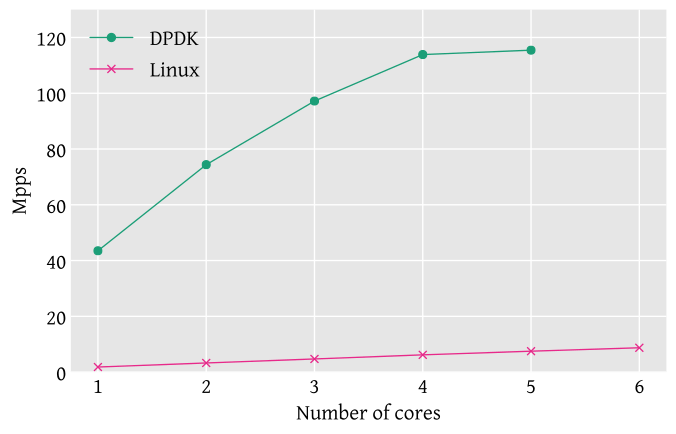
\includegraphics[width=\columnwidth]{pictures/PacketIOComparison.png}
  \caption{パケットI/O処理の比較}
  \label{fig:PacketIOComparison}
\end{figure}

\subsection{DPDKによるパケットI/O処理の問題}
DPDKは特定のCPUコアを専有することによって,NICを常時ポーリングで監視するため,通信負荷が低いときでもCPUリソースを無駄に使用する.文献 \cite{XDP} で調査された,カーネルによるパケットI/O処理とDPDKによるパケットI/O処理のCPU使用率を図\ref{fig:DPDKProblem}に示す.このグラフの横軸は通信負荷,縦軸はCPU使用率を表している.また,緑はDPDKによるパケットI/O処理,青はカーネルによるパケットI/O処理の結果である.グラフから,カーネルによるパケットI/O処理のCPU使用率は通信負荷が高くなるにしたがって徐々に増えていくことが確認できる.それに対して,DPDKによるパケットI/O処理のCPU使用率は通信負荷にかかわらず常に100\%であることが確認できる.

\begin{figure}[htb]
  \centering
  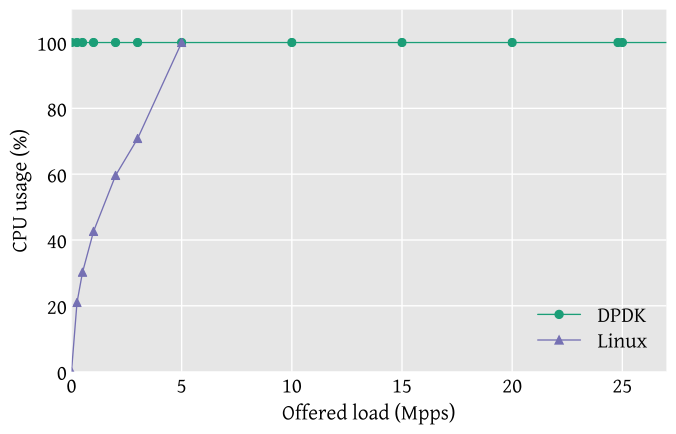
\includegraphics[width=\columnwidth]{pictures/DPDKProblem.png}
  \caption{DPDKによるパケットI/O処理の問題}
  \label{fig:DPDKProblem}
\end{figure}
